\documentclass[a4paper]{article}
\usepackage[T1]{fontenc}
\usepackage[utf8]{inputenc}
\usepackage[MeX]{polski}
\usepackage{pslatex}
\usepackage{graphicx}
\usepackage{tikz}
\usepackage{pgfplots}
\usepackage{anysize}
\usepackage{pgfgantt}
\usepackage{latexsym,amsmath}
\usepackage{hyperref}
\marginsize{2.5cm}{2.5cm}{3cm}{3cm}

\newcommand{\PRzFieldDsc}[1]{\sffamily\bfseries\scriptsize #1}
\newcommand{\PRzFieldCnt}[1]{\textit{#1}}
\newcommand{\PRzHeading}[9]{
%% #1 - nazwa laboratorium
%% #2 - kierunek 
%% #3 - specjalność 
%% #4 - rok studiów 
%% #5 - symbol grupy lab.
%% #6 - temat 
%% #7 - numer lab.
%% #8 - skład grupy ćwiczeniowej
%% #9 - data


\begin{center}
\begin{tabular}{ p{0.32\textwidth} p{0.20\textwidth} p{0.20\textwidth} p{0.1\textwidth} p{0.1\textwidth} }

  &   &   &   &   \\
\hline
\multicolumn{5}{|c|}{}\\[-1ex]
\multicolumn{5}{|c|}{{\LARGE #1}}\\
\multicolumn{5}{|c|}{}\\[-1ex]

\hline
\multicolumn{1}{|l|}{\PRzFieldDsc{Kierunek}}	& \multicolumn{1}{|l|}{\PRzFieldDsc{Specjalność}}	& \multicolumn{1}{|l|}{\PRzFieldDsc{Rok studiów}}	& \multicolumn{2}{|l|}{\PRzFieldDsc{Numer grupy lab.}} \\
\multicolumn{1}{|c|}{\PRzFieldCnt{#2}}		& \multicolumn{1}{|c|}{\PRzFieldCnt{#3}}		& \multicolumn{1}{|c|}{\PRzFieldCnt{#4}}		& \multicolumn{2}{|c|}{\PRzFieldCnt{#5}} \\

\hline
\multicolumn{4}{|l|}{\PRzFieldDsc{Temat Laboratorium}}		& \multicolumn{1}{|l|}{\PRzFieldDsc{Numer prog.}} \\
\multicolumn{4}{|c|}{\PRzFieldCnt{#6}}				& \multicolumn{1}{|c|}{\PRzFieldCnt{#7}} \\

\hline
\multicolumn{5}{|l|}{\PRzFieldDsc{Skład grupy laboratoryjnej}}\\
\multicolumn{5}{|c|}{\PRzFieldCnt{#8}}\\

\hline
\multicolumn{3}{|l|}{\PRzFieldDsc{Prowadzący}}	& \multicolumn{2}{|l|}{\PRzFieldDsc{Data}} \\
\multicolumn{3}{|c|}{\PRzFieldCnt{\PRzFieldCnt{Mgr inż. Radosław Idzikowski} }}		& \multicolumn{2}{|c|}{\PRzFieldCnt{\PRzFieldCnt{#9} }} \\

\hline
\end{tabular}
\end{center}
}
\usepackage{listings}
\usepackage{xcolor} % for setting colors

% set the default code style
\lstset{
    frame=tb, % draw a frame at the top and bottom of the code block
    tabsize=4, % tab space width
    showstringspaces=false, % don't mark spaces in strings
    numbers=left, % display line numbers on the left
    commentstyle=\color{green}, % comment color
    keywordstyle=\color{blue}, % keyword color
    stringstyle=\color{red} % string color
}




\title{Sprawozdanie SPD}
\begin{document}

\PRzHeading{Sterowanie procesami dyskretnymi}{Automatyka i Robotyka}{brak}{3}{9}{Implementacja i analiza efektywności algorytmów dla jednomaszynowego problemu wiTi.}{1}{Maciej Kajdak, Patrycjusz Auguścik}{\today}{}
\pagestyle{empty}
\newpage
\section{Opis problemu}
Podejmowanym problemem jest problem wiTi, czyli problem składający się z liczby n zadań wykonywanych na maszynie. Każdy program charakteryzuje się trzema parametrami:
\begin{itemize}
	\item $p_{i}$ -- czas wykonywania zadania na maszynie
	\item $w_{i}$ -- współczynnik kary za nieukończenie zadania w zadanym terminie
	\item $d_{i}$ -- maksymalny termin wykonanania zadania
\end{itemize}
Implementację zadania przedstawiono na listingu \ref{lst:Zadanie}

\begin{lstlisting}[firstline = 3,label={lst:Zadanie},caption={Implementacja zadania},language=C++]
typedef int TypDanych;

class Zadanie {
private:
    int NumerZadania;
    TypDanych p;
    TypDanych w;
    TypDanych d;

public:
   
    Zadanie(int NumerZadania, TypDanych p, TypDanych w, TypDanych d);

    virtual ~Zadanie();

    // ----------------------------- Operatory, gettery i settery ---------------------------
    int getNumerZadania() const;

    TypDanych getP() const;

    TypDanych getW() const;

    TypDanych getD() const;
};
\end{lstlisting}
Wczytując plik tworzymy \underline{zbiór zadań}, dla którego zaimplementowano algorytmy szeregowania.

Dla zadania nie dopuszcza się przerwania, a dla każdego zadania można naliczyć tzw spóźnienie Tardiness wyrażone wzorem:
\begin{equation}
	T_{i}=max(0,C_{i} - d_{i}),
\end{equation}
gdzie $C_{i}$ to czas zakończenia wykonywania i-tego zadania.


\newpage
\section{Metoda rozwiązania}
Do rozwiązania problemu użyto 3 metod:
\begin{itemize}
	\item Sortowanie względem najmniejszej kary,
	\item Przegląd zupełny,
	\item Algorytm programowania dynamicznego.
\end{itemize}

Dla każdego jako kryterium optymalizacyjne używana była tzw. suma witi przedstawiana wzorem:
\begin{equation}
	\sum_{i=1}^{n}w_{i}T_{i}
\end{equation}
Całe zadanie rozwiązania problemu polega na znalezieniu takiej permutacji zadań na maszynie, aby otrzymana suma była najmniejsza.
\\
\\
\subsection{Sortowanie względem najmniejszej kary}
Jedną z najprostszych metod optymalizacji jest posortowanie zadań względem wybranego parametru lub kilku. Tutaj wybrano sortowanie względem najmniejszej kary. Algorytm znajduje zazwyczaj permutację korzystniejszą od permutacji początkowej jednak nie jest to wynik zadowalający, gdyż otrzymywana suma wiTi niewiele różniła się od tej otrzymanej dla permutacji początkowej.
Implementację algorytmu dla zadania

Zaimplementowany algorytm przedstawiono na listingu \ref{lst:Sort}.
\begin{lstlisting}[firstline = 3,label={lst:Sort},caption={Algorytm Sortowania Bąbelkowego},language=C++]
void ZbiorZadan::sortW() {
    unsigned long n = this->Zbior->size();
    int firstIndex = 0, secondIndex = 0;
    do {
        for (int i = 0; i < n - 1; ++i) {
            firstIndex = (*this->KolejnoscZadan)[i];
            secondIndex = (*this->KolejnoscZadan)[i + 1];
            if ((*this->Zbior)[firstIndex].getW() < (*this->Zbior)[secondIndex].getW()) {
                std::swap((*this->KolejnoscZadan)[i], (*this->KolejnoscZadan)[i + 1]);
            }
        }
        --n;
    } while (n > 1);
}
\end{lstlisting}

\newpage
\subsection{Przegląd zupełny}
Kolejną metodą wyszukiwania optymalnej permutacji zadań na maszynie jest metoda zwana przeglądem zupełnym. Jest to jedna z metod siłowych (ang. brute force), w których próbuje się wszystkich możliwych kombinacji aż trafi się na najlepszą. Jest to metoda znajdująca zawsze optymalne rozwiązanie lecz niestety nie jest efektywna obliczeniowo, ponieważ złożoność takiego algorytmu może być postaci wielomianowej, bardzo często $\Theta(2^{n})$. 
\\
Implementację algorytmu dla zbioru zadań przedstawiono na listingu \ref{lst:PZ}. W implementacji wykorzystano algorytmy z biblioteki standardowej C++, a dokładniej z biblioteki "algorithm", takie jak:
\begin{itemize}
\item next\_permutation, generująca kolejne permutacje w porządku leksykograficznym
\item min\_element, zwracająca iterator do najmniejszego znalezionego elementu w kontenerze
\end{itemize}
\begin{lstlisting}[firstline = 3,label={lst:PZ},caption={Algorytm Przeglądu zupełnego},language=C++]
int ZbiorZadan::PrzegladZupelny() {
    int liczbaZadan = this->Zbior->size();
    unsigned long rozm = silnia(liczbaZadan);
    std::vector<TypDanych> kary(rozm);
    std::vector<int> zadania(liczbaZadan);
    int t = 0, kara = 0, pomoc = 0, minimum = 0;


    for (int i = 0; i < liczbaZadan; ++i)zadania[i] = i;
    do {
        pomoc = 0;
        kara = 0;
        t = 0;
        for (int i = 0; i < liczbaZadan; i++) {
            t += (*this->Zbior)[zadania[i]].getP();
            pomoc = (t - (*this->Zbior)[zadania[i]].getD()) * (*this->Zbior)[zadania[i]].getW();
            if (pomoc > 0) kara += pomoc;
        }
        kary[rozm - 1] = kara;
        --rozm;
    } while (std::next_permutation(zadania.begin(), zadania.end()));
    rozm = silnia(liczbaZadan);

    minimum = *(std::min_element(kary.begin(), kary.end()));
    return minimum;
}
\end{lstlisting}


\newpage
\subsection{Algorytm programowania dynamicznego}
Ostatnią z użytych metod był algorytm programowania dynamicznego, czyli metoda dostarczająca optymalne rozwiązanie w zadowalająco krótkim czasie. Zasadą przyświecającą metodologii dynamicznego programowania jest motto "Dziel i zwyciężaj", które pochodzi od łacińskiej sentencji "Dziel i rządź" (łac. Divide et impera). Jej założeniem jest podzielenie problemu głównego na wiele mniejszych podproblemów, jednak od metody dziel i zwycięzaj programowanie dynamiczne wyróżnia nierozłączność problemów jako spójnej całości, czyli własność optymalnej podstruktury każdego podproblemu. Mówiąc inaczej rozwiązanie optymalne składa się z rozwiązań wielu małych podproblemów, które to rozwiązania muszą być optymalne same w sobie. 
\\
Wynalazcą techniki jest amerykański matematyk Richard Bellman, który za to odkrycie został również uhonorowany w 1979 roku.
Jako, że problem wiTi jest określany jako jeden z problemów NP-trudnych, to rozwiązanie tegoż problemu okazuje się zadaniem nie trywialnym jednak programowanie dynamiczne jest jedną z efektywniejszych technik rozwiązywania ów problemu.
\\
Na listingu \ref{lst:PD} została przedstawiona implementacja algorytmu dla zbioru zadań.

\begin{lstlisting}[firstline = 3,label={lst:PD},caption={Algorytm Programowania Dynamicznego},language=C++]
int ZbiorZadan::AlgProgDynamicznego() {
    int cmax, pomoc;
    int iloscZadan = this->Zbior->size();
    int liczbaPermutacji = std::pow(2, iloscZadan);
    auto *F = new int[liczbaPermutacji];
    auto ost = new int[liczbaPermutacji];
    F[0] = 0;
    for (int index = 1; index < liczbaPermutacji; ++index) {
        cmax = 0;
        F[index] = 999999;
        for (int zad = 0, maska = 1; zad < iloscZadan; ++zad, maska *= 2) {
            if (index & maska) cmax += (*this->Zbior)[zad].getP();
        }
        for(int zad = 0, maska = 1; zad < iloscZadan; ++zad, maska *= 2) {
            if(index & maska) {
                if((pomoc = F[index - maska] + std::max(0, (cmax - 
                    (*this->Zbior)[zad].getD()) * (*this->Zbior)[zad].getW())) <
                    F[index]) {
                    F[index] = pomoc;
                    ost[index] = zad + 1;
                }
            }
        }
    }
    this->PermPD = new std::vector<int>(1);
    int problem=liczbaPermutacji-1, zadanie=ost[problem];
    (*this->PermPD)[0]=zadanie;
    for(int i=1; i<iloscZadan; i++){
        problem=problem & (~(1<<(zadanie-1)));
        zadanie=ost[problem];
        this->PermPD->push_back(zadanie);
    }
    return F[liczbaPermutacji - 1];
} 
\end{lstlisting}
\section{Eksperymenty obliczeniowe}
Obliczenia zostały wykonane na komputerze HP ProBook 455 z procesorem AMD A4-4300M, zintegrowaną kartą graficzną AMD Radeon HD 7420G 8GB RAM oraz dyskiem HDD.
\\
Podczas testowania okazało się, że algorytm przeglądu zupełnego dla instancji większej niż 12 elementów wykonuje się tak długo, że oczekiwanie na zakończenie działania programu jest bezcelowe. dlatego też wyniki dla przeglądu zupełnego ograniczono do pierwszych 3 zbiorów.

\subsection{Analiza jakościowa}
\begin{equation}
PRD(*)=100\%*((wiTi(*)-wiTi_{opt})/wiTi_{opt})
\end{equation}
Wszystkie wyniki zebrano i przedstawiono w tabeli nr \ref{tab:result} gdzie:
\begin{itemize}
\item $n$ - liczba zadań,
\item $PRD_{sortW}(\%)$ - średnie procentowe odchylenie dla algorytmu sortW,
\item $PRD_{PD}(\%)$ - średnie procentowe odchylenie dla algorytmu programowania dynamicznego,
\item $t_{sortW}(s)$ - czas dla algorytmu sortW,
\item $t_{PD}(s)$ - czas dla algorytmu programowania dynamicznego,
\end{itemize}
\begin{table}[h!]
\centering
	\caption{Czas obliczeń oraz PRD dla ustalonej liczby iteracji.}
	\label{tab:result}
	{\begin{tabular}{cccccc}
		\hline
		$n$ &$optimum$&$PRD_{sortW}(\%)$ & $PRD_{PD}(\%)$& $t_{sortW}(s)$& $t_{PD}(s)$ \\
		\hline
       	10 & 1004 & 200 & 0 & 0.004 & 0.441 \\
		11 & 962 & 214 & 0 & 0.004 & 0.839\\
		12 & 915 & 314 & 0 & 0.004 & 1.763\\
		13 & 681 & 459 & 0 & 0.005 & 3.931\\
		14 & 646 & 526 & 0 & 0.006 & 8.364\\
		15 & 310 & 1355 & 0 & 0.006 & 16.89 \\
		16 & 321 & 1873 & 0 & 0.007 & 36.136 \\
		17 & 746 & 787 & 0 & 0.01 & 72.808 \\
		18 & 539 & 1170 & 0 & 0.009 & 160.874 \\
		19 & 688 & 1001 & 0 & 0.013 & 331.032 \\
		20 & 514 & 1523 & 0 & 0.01 & 706.47 \\		
		
		\hline
		\bf{Średnio}& & \bf{0.2225}& \bf{0.2225}& \bf{-5.54}& \bf{-4.34} \\
		\hline
	\end{tabular}}
\end{table}
Dla algorytmu przeglądu zupełnego zawsze (dla zbadanych instancji oraz z definicji dla każdej innej) algorytm znajdował rozwiązanie optymalne, więc z powodu braków w wynikach eksperymentu nie uwzględniono przeglądu zupełnego w tabeli.


\newpage
\subsection{Analiza wydajnościowa}
Do analizy wydajnościowej został wygenerowany wykres zależności czasu od wielkości instancji problemu, a został on przedstawiony na rysunku \ref{fig:wydajnosc}. 
\begin{figure}[h]
	\centering
	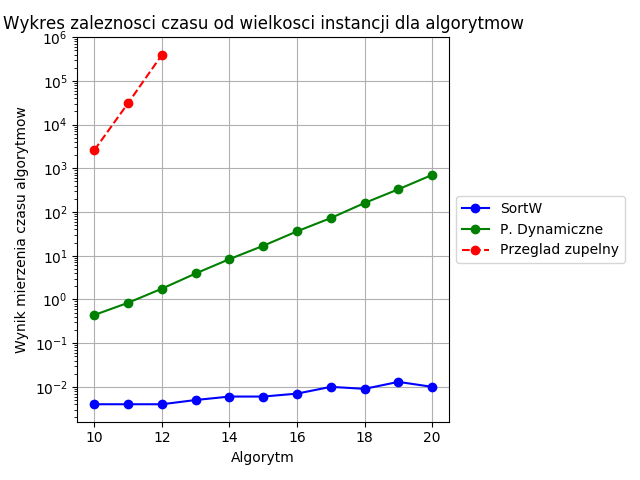
\includegraphics[width=0.8\textwidth]{Figure_1.png}
	\label{fig:wydajnosc}
	\caption{Analiza wydajnosciowa}
\end{figure}

Tutaj załączono wyniki zbadanych instancji metodą przeglądu zupełnego, aby pokazać kontrast na tle pozostałych metod.


\section{Wnioski}
Jak widać przedstawione algorytmy mogą mieć swoje za oraz przeciw. Dla przeglądu zupełnego zaletą jest prostota implementacji oraz działania jednak niewątpliwą wadą jest czas działania w zależności od wielkości problemu. Sortowanie jest, nie da się ukryć, jedną z najgorszych metod szukania optymalnego rozwiązania, gdyż nie najczęściej nie da nam rozwiązania optymalnego mimo, że czas działania, a tym samym złożoność obliczeniowa, jest najmniejszy spośród tutaj przedstawionych. Przegląd zupełny jako przykład metody zachłannej w swojej złożoności bardzo szybko rośnie do ogromnych rozmiarów, najczęściej wykładniczo więc dla bardzo małych instancji może być stosowany, jednak nie jest to polecane. Najlepszym rozwiązaniem wydaje się programowanie dynamiczne i idea rozdzielania problemu głównego na mniejsze podproblemy. Po pierwsze daje ono rozwiązanie optymalne za każdym razem, a po drugie -- robi to w relatywnie krótkim czasie. Jednakowoż trudność zrozumienia działania algorytmu oraz jego implementacji mogą na pierwszy rzut oka odstraszać.


\bibliographystyle{abbrv}
\bibliography{ref}

\end{document}

